% !TEX root = ../Dokumentation.tex
\subsection{Intelligente Systeme}

\subsubsection{Software auf Mini-Computer}
Das Softwarekonzept basiert auf dem MVC\footnote{MVC = Model-View-Control}-Prinzip, wobei sich die View auf einen reinen Debug-Zweck beschränkt. Der Controller kommunziert mit allen Subprozesse und grenzt an die Schnittstelle zur Hardwaresteuerung. Um die Performance des Rasperry Pi möglichst auszunutzen wird mit Threads gearbeitet. Die parallel laufenden Subprozesse sind:

\begin{itemize}
\item Bilderzeugung,
\item Objekterkennung und
\item Fahrbahnerkennung.
\end{itemize}

\begin{figure}[H]
	\centering
	\includegraphics[width=0.8\textwidth]{03_Loesungskonzept/pictures/grobablauf.png}
	\caption{Aktivitätendiagramm Grobablauf}
\end{figure}

Der Zustand des Fahrzeuges wird im Model gespeichert und steht allen Prozessen zur Verfügung. Die Datenstruktur ist dabei so aufgebaut, dass keine Zugriffskonflikte entstehen sollten.\\
Der Controller behandelt alle Anweisungen der Prozesse. Meldet beispielsweise die Objekterkennung einen Container, hat dieser Priorität vor dem normalen Fahren und das Mikrocontroller-Board erhält die entsprechenden Anweisungen. Das folgende Diagramm zeigt eine Gesamtübersicht von den verschiedenen Komponenten.\\[0.2cm]
\begin{figure}[H]
\centering
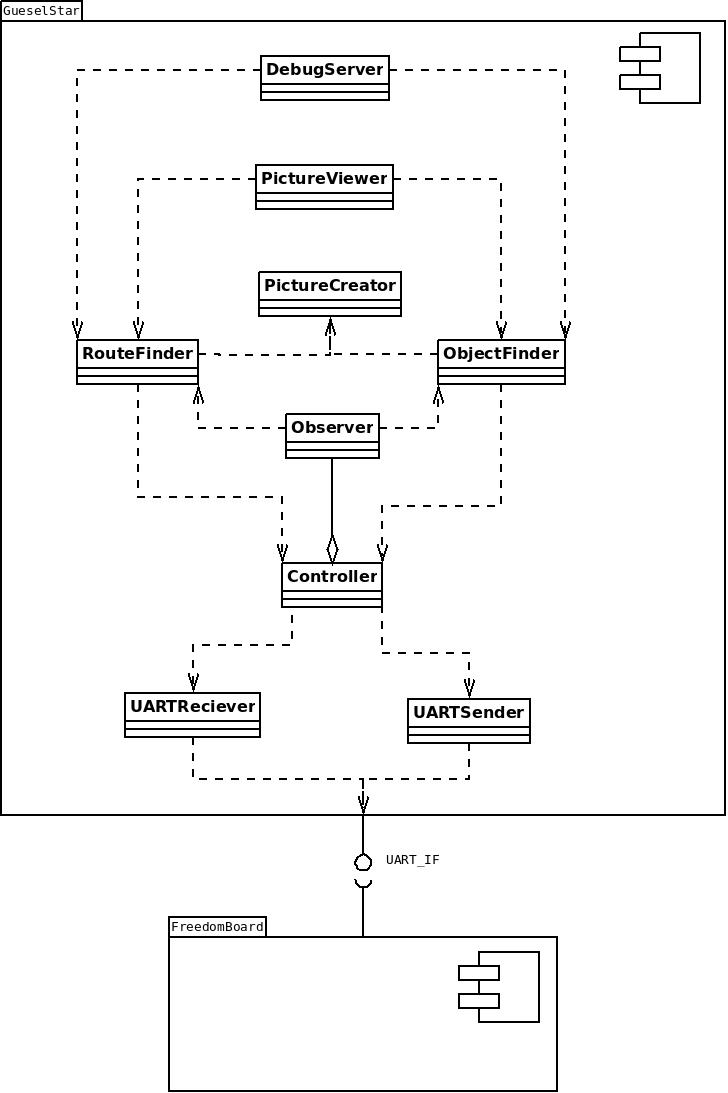
\includegraphics[width=0.8\textwidth]{03_Loesungskonzept/pictures/Komponentendiagramm_detailliert_v2.jpeg}
\caption{Komponentendiagramm}
\end{figure}

\textbf{Debug-View}\\[0.2cm]
Um während der Implementierungs-Phase der geschriebene Code zu testen wurde eine Debug-View entwickelt. Mit dieser kann auf den Debug-Server, welcher auf dem Raspberry Pi gestartet wird, zugegriffen werden. Nach einer erfolgreichen Verbindung werden die aufgenommenen Bilder vom Server an den Client (GueselStarObserver) gesendet.

\begin{figure}[H]
\centering
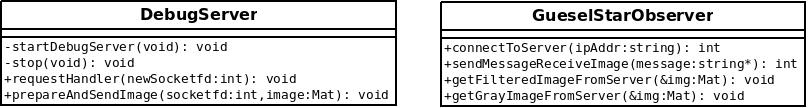
\includegraphics[width=0.8\textwidth]{03_Loesungskonzept/pictures/DebugView.jpeg}
\caption{Debug-View}
\end{figure}

Die Kommunikation zwischen Server und Client läuft über TCP/IP. Auf dem Server wird ein Server-Socket geöffnet, auf welches sich der Client verbinden kann.

\textbf{Konfiguration}\\[0.2cm]
Neu geschriebener Code benötigt einen erneuten Build. Um einen neuen Build, welcher Zeit benötigt, zu unterbinden wurde eine Konfigurations-Datei erstellt, in welcher alle benötigten Parameter angepasst werden können. Das Einlesen der Konfiguration erfolgt über einen selbstentwickelten Parser und wird anschliessend in einem Objekt der Klasse "PRENConfiguration" abgespeichert.

\begin{figure}[H]
\centering
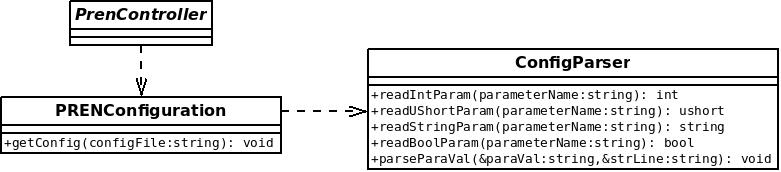
\includegraphics[width=0.8\textwidth]{03_Loesungskonzept/pictures/Configuration.jpeg}
\caption{Konfiguration}
\end{figure}
 
%***************************
\subsubsection{Software auf Mikrocontrollerboard}

\textbf{SW Architektur}\\[0.2cm]
Auf dem Mikrocontroller (Freedomboard KL25Z) wurde mit dem Betriebssystem FreeRTOS gearbeitet. Dies ermöglicht die Erstellung von verschiedenen Tasks. Dies erlaubt eine bessere Trennung der einzelnen Softwarekomponenten und erleichtert das Programmieren. Die verschiedenen Tasks wurden bereits im PREN1 geplant und nun im PREN2 umgesetzt. 
Hier eine Übersicht der Tasks und Events:

\begin{figure}[H]
	\centering
	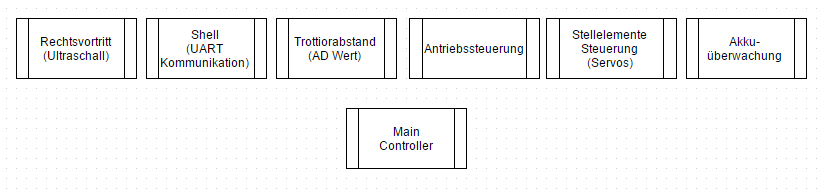
\includegraphics[width=0.9\textwidth]{03_Loesungskonzept/pictures/MC_Tasks.png}
	\caption{Übersicht MC Tasks}
\end{figure}
In den folgenden Abschnitten werden kurz auf die einzelnen Tasks und Events eingegangen. Dies dient jedoch nur der Übersicht.\\
\textbf{Controller}\\[0.2cm]
Dieser Task steuert das Freedomboard. Das heisst konkret, dass dieser Task das initialisieren, fahren, aufladen, entladen  und beenden des Programmes zuständg ist. Dies ist über eine FineState Maschiene realisiert, welche bei besonderen Events den State wechselt. Ein besonderer Event ist zum Beispiel das Startkommando über die Kommunikation oder eine Unterspannung am Akku.\\[0.2cm]
\textbf{Kommunikation}\\[0.2cm]
Dieser Task übernimmt die Auswertung der erhaltenen Kommandos über die UART Schnittstelle. Dies geschieht über eine sogenannte Parsertabelle. In dieser Parsertabelle können beliebig weitere Kommandos (Funktionen) hinzugefügt werden. Dieser Task wird alle 10ms aufgerufen, da die Kommunikation mit dem Raspberry Pi möglichst schnell funktionieren soll.\\[0.2cm]
\textbf{Analog-Digitalwandlung}\\[0.2cm]
Dieser Task holt und verarbeitet die Daten aus dem Analog Digitalwandler des KL25Z. Das heisst konkret es werden beide Akku Spannungen ausgelesen und überwacht. Zudem wird der Widerstandswert des Flexsensensors eingelesen und damit der Abstand zum Gehsteig berechnet. Zur Akkuüberwachung folgen weiter im Text weitere Informationen.\\[0.2cm]
\textbf{Geschwindigkeitsregelung}\\[0.2cm]
Der Geschwindigkeitsregelungstask regelt die Geschwindigkeit des DC-Antriebmotors. Dies geschieht über einen PID Regler. Dieser wurde vom Modul Mikrocontrollertechnik an der Hochschule Luzern übernommen und nach den eigenen Bedürfnissen angepasst. Wie die PID Werte berechnet wurden und der Regelkreis aussieht wird noch separat erläutert.\\[0.2cm]
\textbf{Ultraschall}\\[0.2cm]
Dieser Task steuert den Ultraschallsensor an. Dies wurde nach einem Tutorial von mcuoneclipse.com realisiert und auf die Softwareumgebung noch weiter angepasst.\\[0.2cm]
\textbf{Master check}\\[0.2cm]
Dieser Task ist die Lebensversicherung des Fahrzeugs. Hier wird überprüft ob der Master (Raspberry Pi) noch angeschlossen und Funktionstüchtig ist. Wenn das Mikrocontrollerborad nicht innerhalb von wenigen Sekunden eine Bestätigungsmeldung des Masters bekommt, wird das Freedomboard in den Beendet Modus wechseln und fährt somit nicht unkontrolliert herum. \\[0.2cm]
\textbf{Event}\\[0.2cm]
Die Events treten unregelmäßig und ungeplant auf. Diese unterbrechen das normale Programm (Interrupt) und führen einen eigenen kurzen Programmcode aus. Dies ist bei den im Bild aufgeführten Funktionen der Fall.\\[0.2cm]
%***************************
\subsubsection{Schnittstellen}